\chapter{Compilers and Virtual Machines for Java-like languages in the
  Safety-critical Domain}
\label{literature-review-chapter}

This chapter begins with a discussion of why Java is being used in
safety-critical systems and the need for a specialised version of Java
for use in that area.
Then, in Section~\ref{scj-section} we cover the variant of Java
developed for safety-critical systems, how it differs from standard
Java and why a specialised virtual machine is required, before
discussing some of the existing virtual machines for that variant in
Section~\ref{virtual-machines-section}.

In Section~\ref{compiler-correctness-section} we survey some of the
literature on compiler correctness, and discuss the two main
approaches in Sections~\ref{commuting-diagram-subsection} and
\ref{algebraic-approach-subsection}, before seeing how the techniques
of compiler correctness have been applied to Java-like languages in
Section~\ref{java-compiler-correctness-subsection}.

In Section~\ref{circus-section}, we give an overview of the \Circus{}
specification language used for our virtual machine specification,
before concluding in Section~\ref{final-considerations-section}.

\section{Java for Safety-critical systems}
\label{java-safety-critical-section}

% provide motivation for SCJ, mentioning standard Java and RTSJ

In recent years Java has increasingly been considered as a language
for writing safety-critical software.
Other languages that are generally used in the safety-critical domain
are C/C++ and Ada; C and C++ impose challenges concerning reliable use
at the highest levels of safety~\cite{kornecki2009}, and the number of
Ada programmers is not very large~\cite{bissyande2013}.
While Java has not traditionally been seen as a language for
safety-critical systems, it was originally developed for the area of
embedded systems, particularly for use in television set-top boxes,
and has seen renewed interest in its use in embedded systems after
gaining popularity in programming for the
internet~\cite{mulchandani1998}.

There are, however, several issues with standard Java that make it
unsuitable for safety-critical systems.
Many safety critical systems are also real-time systems, which are
required to be predictable in their scheduling and use of memory.
However, standard Java uses a garbage-collected memory model, which
makes it hard to predict when memory may be freed or how long the
process of freeing memory may take.
Standard Java's thread model also lacks the predictability and control
that is required in real-time systems.

To rectify these problems the Real-Time Specification for Java
(RTSJ)~\cite{gosling2000} was created; it augments Java's memory and
scheduling models with a system of scoped memory areas and a
preemptive priority scheduler.
RTSJ also allows for the standard Java models to be used alongside its
own, making it suitable for a wide range of different real-time
applications.
On the other hand, this makes it hard to certify RTSJ applications and
thus renders the RTSJ unsuitable for use in the safety-critical
domain.

In order to allow certifiable safety-critical systems in Java, the
Safety-Critical Java (SCJ)~\cite{locke2013} specification was
developed.
SCJ is a subset of the RTSJ that leaves out the features from standard
Java that are difficult to certify such as the garbage collector.
SCJ also provides annotations that allow memory usage to be more
easily checked.
We discuss SCJ in more detail in the next section.

\section{Safety-Critical Java}
\label{scj-section}

SCJ removes the aspects of the RTSJ that make certification difficult,
including standard Java threads and the garbage collector.
This leaves scheduling and memory management models that are very
different to the models for standard Java and that, therefore, require
specialised virtual machines to support them.

SCJ defines three compliance levels to which programs and
implementations may conform.
Level 0 is the simplest compliance level.
It is intended for programs following a cyclic executive approach.
Level 1 lifts several of the restrictions of level 0, allowing
handlers that may trigger in response to external events and preempt
one another.
Level 2 is the most complex compliance level, allowing access to
real-time threads and suspension via \texttt{wait()} and
\texttt{notify()}.  

An SCJ program consists of one or more missions, which are collections
of schedulable objects that are scheduled by SCJ's priority scheduler.
Missions are run in an order determined by a mission sequencer
supplied by an SCJ program.
Running a mission proceeds in several phases, as shown in
Figure~\ref{phases-diagram}.

\begin{figure}[ht]
  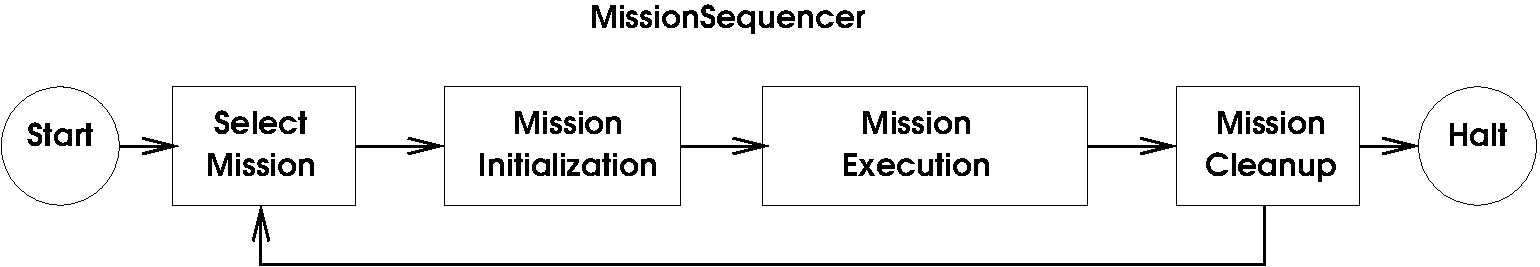
\includegraphics[width=\textwidth]{phases.pdf}
  \caption{A diagram showing the phases of SCJ mission execution}
  \label{phases-diagram}
\end{figure}

The fist phase is initialisation, which consists of setting up the
schedulable objects controlled by the mission and creating any data
structures required for the mission.
Then the mission is executed by starting each of the schedulable
objects in the mission and waiting for a request to terminate the
mission.
When the mission is requested to terminate, each of the schedulable
objects in the mission is terminated and the mission's memory is
cleared.

The schedulable objects within a mission are asynchronous event
handlers that are released either periodically, at set intervals of
time, aperiodically, in response to a release request, or once at a
specific point in time (though handlers that are released once can
have a new release time set, allowing them to be released again).
At level 2 real-time threads are also allowed, which run continuously
from when they start until they finish, unless they are suspended or
interrupted by another schedulable object.

Each schedulable object has a priority and the highest priority object
that is eligible to run at each point in time is the object that runs.
This allows for simpler reasoning about order of execution and allows
for more urgent tasks to preempt less urgent tasks.

SCJ allows for assigning schedulable objects to ``scheduling
allocation domains'', where each domain consists of one or more
processors.
At Level 1, each scheduling allocation domain is restricted to a
single processor.
Hence, in scheduling terms, the system is fully partitioned.
This allows for mature single processor schedulability analysis to be
applied to each domain (although the calculation of the blocking times
when accessing global synchronised methods are different than they
would be on a single processor system due to the potential for remote
blocking~\cite{davis2011}).

SCJ deals with memory in terms of memory areas, which are Java objects
that provide an interface to blocks of physical memory called backing
stores.
Memory allocations in SCJ are performed in the backing store of the
memory area designated as the allocation context.
Each schedulable object has a memory area associated with it that is
used as the allocation context during a release of that object, and is
cleared after each release.
Each mission also has a mission memory area that can be used as an
allocation context by the schedulable objects of that mission, to
provide space for objects that need to persist for the duration of the
mission or to be shared between the schedulable objects.
The amount of memory required for the mission memory must be computed
ahead of time and specified by the programmer as part of writing the
mission, though there has been some work on automated computation of
worst case memory use for SCJ programs~\cite{andersen2013}.
There is also an immortal memory area where objects can be allocated
if needed for the entire running of the program (they are never
freed).
SCJ places restrictions on which objects an object may point to, so as
to avoid dangling pointers from being created.
Some examples of valid and invalid object references for some
asynchronous event handlers are shown in
Figure~\ref{stacks-areas-diagram}.

\begin{figure}[ht]
  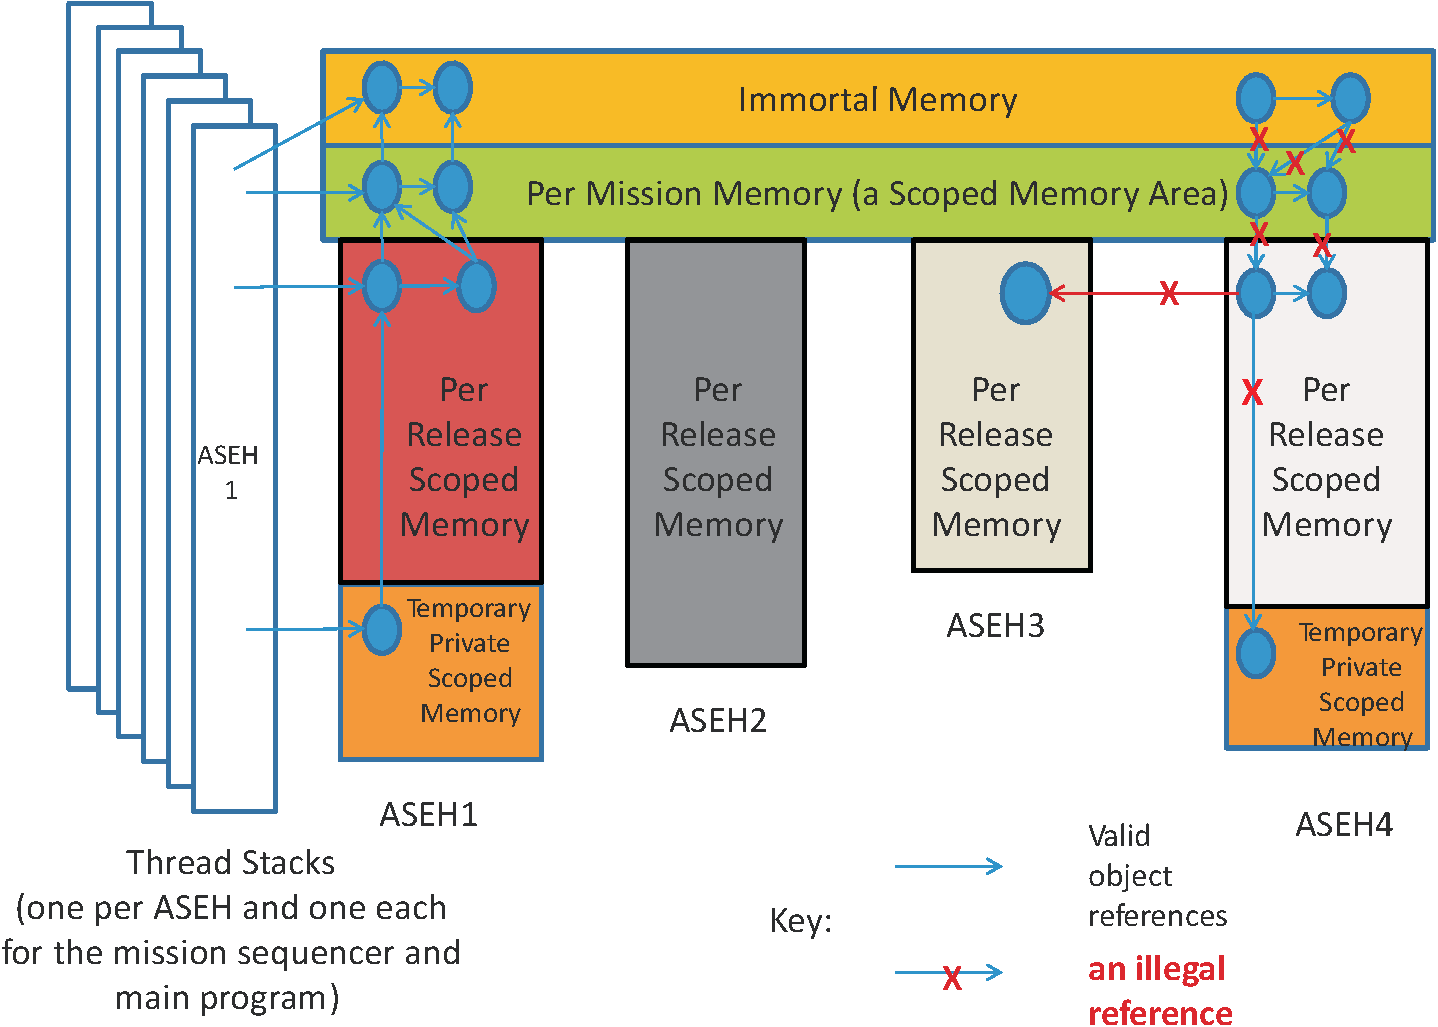
\includegraphics[width=\textwidth]{Stacks-Areas.pdf}
  \caption{An example of the layout of memory areas for four
    asynchronous event handlers (ASEHs), showing possible valid and
    invalid references between them}
  \label{stacks-areas-diagram}
\end{figure}

This system of memory areas makes it easy to predict when memory is
freed.
It is not supported by standard JVMs as they do not provide memory
outside of the heap for allocation and lack a notion of allocation
context.
The SCJ memory manager also needs to provide a means of accessing raw
memory for the purposes of device access, but that section of the SCJ
standard is not yet finalised so we will not cover it here.
It can, however, be seen that any system of raw memory access is not
supported by most standard JVMs.

Moreover, dynamic class loading is not allowed in SCJ; all classes
used by the program must be loaded when the program starts.
This is because dynamic class loading may introduce time overheads
that are hard to predict and additional code paths that complicate
certification.
Finally, SCJ also disallows object finalisers as it is not always easy
to predict when they are run.

\section{Virtual Machines for Safety-Critical Java}
\label{virtual-machines-section}

% one subsection per machine

Because of the novel features of SCJ, briefly described in the
previous section, a specialised virtual machine that provides support
for allocation in memory areas and preemptive scheduling is required
for SCJ.
Although SCJ is a relatively recent development there have been
various virtual machines created for SCJ or variations of SCJ,
including icecap HVM~\cite{sondergaard2012}, Fiji VM~\cite{pizlo2009},
OVM~\cite{armbruster2007}, HVM\textsubscript{TP}~\cite{luckow2014} and
PERC Pico~\cite{atego2015, richard2010}.
These are each described in the following subsections.

\subsection{icecap HVM and HVM\textsubscript{TP}}

The icecap hardware-near virtual machine (HVM) was created as part of
the Certifiable Java for Embedded Systems Project~\cite{schoeberl2014}
and provides an open-source implementation of SCJ targeted at embedded
systems.
The approach taken by the HVM is one of precompiling Java bytecode to
C in order to allow for faster running programs with fewer memory
resources.
It includes an implementation of the SCJ libraries that covers most of
SCJ level 2, though only for a single processor implementation.
This implementation, however, cannot be easily decoupled from the
virtual machine itself.

The icecap HVM also provides a lightweight Java bytecode interpreter
and allows for interpreted code to be mixed with compiled code.
The reason for this is that the bytecode together with the interpreter
can often be smaller than the compiled code, though there is a
tradeoff for speed.
HVM\textsubscript{TP} is a modification of the icecap HVM's bytecode
interpreter to improve time predictability and ensure that bytecode
instructions are executed in constant time, which is important for
ensuring real-time properties of the system hold.

\subsection{Fiji VM}

Fiji VM is a proprietary Java implementation designed to run on
real-time embedded systems.
Similarly to the icecap HVM, Fiji VM uses the strategy of compiling to
C in order to improve performance.
However, Fiji VM is not specifically targeted at SCJ and works with a
range of libraries, including SCJ, RTSJ and the standard Java
libraries.
Fiji VM does have the advantage of high portability and multiprocessor
support, which is lacking in many other SCJ virtual machines.

The fact that Fiji VM works with the SCJ libraries and supports the
scoped memory model means it can run SCJ programs.
It does not necessarily support all aspects of SCJ properly though.

\subsection{OVM}

OVM was created at Purdue University as part of the PCES
project~\cite{baker2006}, to provide a virtual machine that can
execute real-time Java programs with a high level of performance on
embedded systems.
Similar to Fiji VM and icecap HVM, OVM follows the principle of
precompiling code for performance reasons, but translates Java to C++
instead of bytecode to C.

OVM also differs from the icecap HVM and Fiji VM in that it predates
SCJ.
It is written to implement the RTSJ, though it can still support SCJ
programs; indeed, an SCJ implementation for OVM was later
created~\cite{plsek2010}.
However, OVM does not appear to have kept up with more recent changes
to the draft SCJ standard.
OVM is, like icecap HVM, but unlike Fiji VM, single processor.

\subsection{PERC Pico}

PERC Pico is a product of Atego based on early ideas for SCJ, but uses
its own system of Java metadata annotations to ensure the safety of
scoped memory.
This systems of annotations provides additional information about how
memory is used so that it can be checked.
Similarly to other SCJ virtual machines, PERC Pico allows for
precompilation of Java code but targets executable machine code rather
than an intermediate programming language.
The metadata annotations are used to guide the compiler to produce
code that uses the correct scoped memory.
PERC Pico does not support the current SCJ standard, though it has
been suggested that it could be modified to do so~\cite{nilsen2011}.

To summarise, as far as we are aware there is one publicly available
virtual machine that has kept up with the developing SCJ
specification, the icecap HVM.
This is and, typically, virtual machines for SCJ will be, designed to
be very small and fast so as to be able to run on embedded systems.

As can be seen from the preceding discussion, a common technique to
run Java programs on embedded systems is to precompile them to native
code.
This means compiler correctness techniques must be considered in
verification of such a virtual machine; these techniques are discussed
in the next section.

\section{Compiler Correctness}
\label{compiler-correctness-section}

Due to the importance of compiler correctness, there has been much
research over the years in this area.
Most of the work done follows a similar approach, which we will term
the commuting-diagram approach as it is based on showing that a
particular diagram commutes.
We will discuss the commuting diagram approach in
Section~\ref{commuting-diagram-subsection}.

An alternative approach to compiler verification is the algebraic
approach developed in the early 90s.
It is based on the concepts of refinement calculi designed for
deriving software from specifications of behaviour.
We will explain the algebraic approach in
Section~\ref{algebraic-approach-subsection} and discuss how it differs
from the commuting-diagram approach.

We finish in Section~\ref{java-compiler-correctness-subsection} by
reviewing some of the literature on correctness of compilers for
Java-like languages.
We explain how the techniques of compiler correctness have been
applied in the case of Java and compare the different approaches.

\subsection{Commuting-diagram Approach}
\label{commuting-diagram-subsection}

Much of the work on compiler correctness can be seen as following the
approach identified by Lockwood Morris~\cite{morris1973}, and later
refined by Thatcher, Wagner and Wright~\cite{thatcher1979}.
The approach is essentially that a compiler correctness proof is a
proof that the diagram shown in Figure~\ref{commuting-diagram}
commutes, that is, $\gamma \circ \psi = \phi \circ \epsilon$.

\begin{figure}[ht]
  \begin{center}
    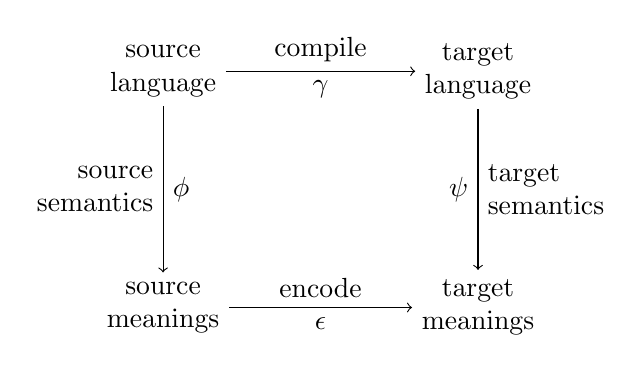
\begin{tikzpicture}
      \node[align=center] (S) at (0cm,3cm) {source\\language};
      \node[align=center] (T) at (4cm,3cm) {target\\language};
      \node[align=center] (M) at (0cm,0cm) {source\\meanings};
      \node[align=center] (U) at (4cm,0cm) {target\\meanings};
      
      \path (S) edge[->] node[align=center, above] {compile}
      node[align=center, below] {$\gamma$} (T); \path (S) edge[->]
      node[align=right, left] {source\\semantics}
      node[align=center,right] {$\phi$} (M); \path (T) edge[->]
      node[align=left, right] {target\\semantics} node[align=center,
      left] {$\psi$} (U); \path (M) edge[->] node[align=center, above]
      {encode} node[align=center, below] {$\epsilon$} (U);
    \end{tikzpicture}
  \end{center}
  \caption{The commuting diagram used in the traditional approach to
    compiler verification}
  \label{commuting-diagram}
\end{figure}

Lockwood Morris had the corners of the diagram as algebras, rather
than merely sets, with the functions between them being homomorphisms
in order to add additional structure to the proof.
This differs from the approach of some earlier works, particularly the
earliest work by McCarthy and Painter~\cite{mccarthy1967}, and instead
follows work such as that of Burstall and Landin~\cite{burstall1969}.

McCarthy and Painter's work featured a simple expression language with
addition, natural numbers and variables.
This was compiled to a simple 4-instruction single-register machine.
The arrows of the diagram were simple functions, rather than
homomorphisms, and the proof was performed using induction over the
source language.
This work laid the foundation for the study of compiler correctness.

Burstall and Landin show correctness of a compiler for the same source
and target languages as McCarthy and Painter; they use a more
algebraic approach that better matches what Lockwood Morris later
suggested.
Burstall and Landin's approach involved representing the source and
target languages, and their meanings, as algebras, with the
compilation functions as homomorphisms.
They target several intermediate machines in the proof of correctness.
Viewing the languages as algebras allows for simpler proofs as some of
the arrows of the commuting diagram can be wholly or partially derived
from the algebraic structure.
It was this goal of simplifying the proofs that led Lockwood Morris to
advocate the use of algebras and homomorphisms.

The overall goal of pursuing formal proofs of compiler correctness, as
proposed by McCarthy and Painter~\cite{mccarthy1967}, is to allow
machine-checked proofs of program correctness.
There has been work in that area, the earliest of which is that by
Milner and Weyhrauch~\cite{milner1972} who show the correctness of an
ALGOL-like language.
The proof of correctness was partially mechanised in the LCF theorem
prover~\cite{milner1972a} and the authors were of the opinion that the
proof was feasible and could be completed relatively easily.
A point to note is that Milner and Weyhrauch acknowledged the need for
some way of structuring the proof in order to make it amenable to
machine-checking.
This gives further support to the algebraic commuting diagram approach
advocated by Lockwood Morris.
Indeed, Milner and Weyhrauch explicitly followed that approach as they
were in discussions with Lockwood Morris.

One advantage to making proofs easily machine-checkable, apart from
the added certainty that the proof is correct, is that working
compilers can be created from the machine-checked proofs.
Code generation facilities are available with many theorem provers
such as those of Isabelle/HOL~\cite{haftmann2007} and
Coq~\cite{letouzey2003, letouzey2008}.
The fact that the commuting-diagram approach involves treating the
compilation as a function between algebras representing the source and
target languages fits well with this idea.
In this case, there is then a function defined in the mechanised logic
for the purposes of conducting proofs about it that can be readily
extracted to executable code.

The commuting-diagram approach has been followed in much of the
literature through the years, though not always with the algebraic
methods recommended by Lockwood Morris.
The basic structure of the commuting diagram is a fairly natural
approach to take, as seen by work such as that of the ProCoS
project~\cite{buth1992}.

Another piece of work that follows the commuting diagram approach is
that of Polak~\cite{polak1981}, who states that he is more interested
in verification of a ``real'' compiler rather than ``abstract code
generating algorithms'', and shows the correctness of a compiler for a
Pascal-like language.
This work focuses much more on pragmatic applications of the
commuting-diagram approach, leaving behind the algebraic ideas of
earlier papers.
It sets a precedent for a simpler verification approach based on
considering the functions in the commuting diagram.

The commuting diagram has also been used in recent work, some of the
most successful of which is that of CompCert~\cite{leroy2009a,
  leroy2009b, leroy2012}.
This is a project to create a fully verified realistic compiler for a
subset of C, using the theorem prover Coq~\cite{coq2004}.

There is also recent variation of the commuting-diagram approach, 
based on an operational semantics of the source
language~\cite{bahr2015}.
In this work, the operational semantics of the source language and
a way of relating the source and target semantics are used to derive a
different operational semantics of the source language acting on the
state of the target machine.
The semantics of the target language are then identified as part of
that operational semantics and it is transformed to extract a
compilation function.
This approach may be viewed as variant of the commuting-diagram
approach in which the compilation function is derived from the source
and target semantics and the relationship between them, rather than
being verified by those elements of the commuting-diagram.

\subsection{Algebraic Approach}
\label{algebraic-approach-subsection}

The second main approach to showing correctness of compilers is the
algebraic approach proposed by Hoare in 1991~\cite{hoare1991}, and
further developed by Sampaio~\cite{hoare1993, sampaio1993,
  sampaio1997}.
We note that the algebraic approach discussed in this section is
largely unrelated to the algebraic commuting-diagram approaches
mentioned in the previous section.

The algebraic approach to compilation derives from the concepts of
algebraic reasoning about programs and program refinement.
These concepts come from the idea, proposed by Hoare in
1984~\cite{hoare1984}, that programs can be thought of as predicates
and so the laws of predicate logic can be used to construct laws for
reasoning about programs~\cite{hoare1987}.
As an example of such a law for reasoning about programs, we present
below associativity of sequential composition,
Equation~\eqref{seq-comp-assoc}, and left and right unit of sequential
composition, namely, the program $\Skip$ that does nothing,
Equation~\eqref{skip-comp-identity}.
\begin{equation}
  \label{seq-comp-assoc}
  P;(Q;R) = (P;Q);R
\end{equation}
\begin{equation}
  \label{skip-comp-identity}
  P;\Skip = \Skip;P = P
\end{equation}

The notion of refinement is central to the algebraic approach to
compilation.
Refinement calculi have been developed, independently, by
Back~\cite{back1981}, Morris~\cite{morris1987} and
Morgan~\cite{morgan1990}, following from earlier concepts of program
transformation~\cite{bauer1976, balzer1976, standish1976, arsac1979}.
The basic idea is that there is a relation between programs that
captures the idea of one program being ``at least as good as'' another
or, to put it more precisely, at least as deterministic as another.
Languages and laws for reasoning about programs with this notion of
refinement can then be used to develop programs from specifications.
This means that certain aspects of a system can have a
nondeterministic specification and several different implementations
can refine that specification.

In using refinement to show the correctness of a compiler, the laws of
the specification language can be used to prove compilation refinement
laws.
These compilation laws can be used to transform the source programs
into some normal form that represents an interpreter for the target
language running the target code.
In other words, the code output by the compiler, when executed by on
the target machine, must be a refinement of the source program.
The compilation laws can be used to prove this refinement and at the
same time generate the target code.

As an example, consider the following refinement in which a simple
program that performs some arithmetic and stores the results into
variables is refined by a normal form representing the target machine
and code.
The symbol $\circrefines$ represents the refinement relation here.
\begin{equation}
  \circvar x, y, z \circspot x := (x + 5) \times (y + z) ; z := z + 1
  \circrefines
  \begin{aligned}
    &\circvar A, P, M \circspot P := 1; \circdo \\
    &\quad            P=1  \then A,    P := M[2],          2 \\
    &\quad \extchoice P=2  \then A,    P := A + M[3],      3 \\
    &\quad \extchoice P=3  \then M[4], P := A,             4 \\
    &\quad \extchoice P=4  \then A,    P := M[1],          5 \\
    &\quad \extchoice P=5  \then A,    P := A + 5,         6 \\
    &\quad \extchoice P=6  \then A,    P := A \times M[4], 7 \\
    &\quad \extchoice P=7  \then M[1], P := A,             8 \\
    &\quad \extchoice P=8  \then A,    P := M[3],          9 \\
    &\quad \extchoice P=9  \then A,    P := A + 1,         10 \\
    &\quad \extchoice P=10 \then M[3] := A,                11 \\
    &\circod ; \{ P = 11 \}
  \end{aligned}
\end{equation}
The normal form represents the behaviour of an interpreter for the
target code running in a target machine whose structure is defined
by the variables A, P, and M.
The variable $A$ represents a general-purpose register of the target
machine, $P$ represents the program counter of the target machine, and
$M$ is an array representing the memory of the target machine.
The normal form consists of a program that initialises $P$ to 1 and
then enters a loop in which the operation performed on each iteration
is dependent on the value of $P$.
The loop is exited when $P$ is set to a value for which there is no
operation and it is asserted that $P$ will be equal to 11 at the end
of the program.
Each of the statements of the source program corresponds to several
operations in the normal form as complex expressions are broken down
into simpler expressions that can be handled by instructions of the
target machine.

The compilation proceeds by first applying rules to simplify the
assignment statements.
The register $A$ is introduced at this stage by splitting assignments
of expressions to variables into two assignments that transfer the
values to and from $A$.
In this way, the assignments are transformed for the target machine
that only has instructions involving registers.
Particularly complex expressions such as $(x + 5) \times (y + z)$ are
handled by storing intermediate results in temporary variables.
In this case the result of the expression $y + z$ is placed in a
temporary variable when $P = 3$.
The variables used in the source program and introduced compilation
are later replaced with locations in the memory array $M$ in a data
refinement step.
This causes the variables $x$, $y$ and $z$ to be replaced with $M[1]$,
$M[2]$ and $M[3]$ respectively.
The temporary variable introduced to store the result of $y + z$ is
similarly replaced with $M[4]$.

Each of the assignment statements from is then refined by a normal
form with an explicit program counter $P$, that is incremented as part
of the assignment operation.
These normal forms are then combined together by the refinement rule
for sequential composition to create the normal form of the full
program.
The update of the program counter in this program is quite simple but
more complex updates would occur for conditionals or loops.

The power of the algebraic approach is that the compilation of
individual elements of the source language can be specified and proved
separately in different refinement laws.
The compilation can also be split into stages, with a set of
refinement laws for each stage to modularise the compilation.
The separate refinement laws can then be combined to form a
compilation strategy.

The first major work done using the algebraic approach was that of
Sampaio~\cite{sampaio1993}, who used it to specify a correct compiler
for a simple language that, nonetheless, covers all the constructs
available in most programming languages.
The target machine Sampaio used was a simple single-register machine
that bears similarity to most real processor architectures.
He mechanised the compiler in the OBJ3 term rewriting
system~\cite{goguen1988}, showing that working compilers can be easily
created from specifications using the algebraic approach.
However, the algebraic laws Sampaio used to prove correctness of the
compiler were taken as axioms.
Sampaio notes that they could be easily proved given a semantics for
the reasoning language.

Though there has not been much work done using the algebraic approach,
we single out the work of Perna~\cite{perna2010, perna2011}, showing
correctness of a compiler for a hardware description language.
The compilation takes high-level descriptions of hardware written in
Handel-C and transforms them into systems of basic hardware components
connected by wires.
The algebraic approach works well here as the target language is a
subset of the source language, albeit in a different form.
Perna was able to handle features not covered by most other works on
hardware compilation, such as parallelism with shared variables.
Also, whereas Sampaio took the basic algebraic laws as axioms, Perna
proved the laws from a semantics given using the Unifying Theories of
Programming (UTP) model~\cite{hoare1998}.
There has also been work on the correctness of Java compilers using
the algebraic approach.
This is considered in the next section, where we consider compiler
correctness for Java-like languages.

\subsection{Correctness of Java Compilers}
\label{java-compiler-correctness-subsection}

The popularity of Java has meant that there has been plenty of work on
formalising Java and the JVM~\cite{hartel2001}, but there have been
relatively few works on formally verified compilers for Java-like
languages.
However, the work that has been done uses both of the two main
approaches and covers most of the features of Java.

Some of the earliest and most thorough work is that by S\"{a}rk,
Schmid and B\"{o}rger~\cite{stark2001}, who formalise most of Java and
the JVM before specifying and showing the correctness of a compiler
for Java.
The approach taken by them uses Abstract State Machines (ASMs) to
specify the source and target languages.
The ASMs give an operational semantics to Java and the JVM, describing
how each construct affects the running of the program.
The languages are each specified by multiple ASMs, beginning with an
imperative core, then adding classes, objects, exceptions and,
finally, threads.

Although this approach is called the ASM approach, it becomes clear
from the definition of compiler correctness given in terms of a
mapping between ASMs that this work ultimately follows the
commuting-diagram approach.
This work leaves parts of the proof incomplete (in particular,
compilation of threads is not addressed) and applies to an old version
of Java.
This is, nevertheless, an admirable attempt at producing a verified
Java compiler.

Work has also been done by Duran following the algebraic
approach~\cite{duran2005, duran2010}.
Duran's work specifies a compiler for a language called Refinement
Object-Oriented Language (ROOL)~\cite{borba2000}, which was created
for reasoning about object-oriented languages and bears much
similarity to Java.
ROOL features constructs for specifying and reasoning about programs
as well as object-oriented programming language constructs.
This means that the there are algebraic laws for ROOL, from which the
rewrite rules that form the basis of the algebraic approach can be
proved.
Duran's work adds further phases to Sampaio's compilation strategy in
order to deal with the object-oriented features, but does not consider
some other aspects of Java such as exceptions and threads.
Duran notes that other work has addressed some of those issues.

While the two works already discussed were not machine checked, there
have also been compiler correctness proofs for Java-like languages in
the Isabelle/HOL proof assistant.
The first of these was by Strecker~\cite{strecker2002}, showing
correctness of a compiler for a subset of Java called $\mu$Java, which
already had a formalisation of its semantics in
Isabelle/HOL~\cite{nipkow2000}.
This work was followed by Klein and Nipkow's work on a compiler for a
slightly larger subset of Java called Jinja~\cite{klein2006}, which
added exception handling.
Finally, Lochbihler~\cite{lochbihler2010} added threads to Jinja and
showed correctness of compilation for Java concurrency.
It is notable that this is the only work on Java compilation that
properly addresses concurrency.
All of these works follow the commuting diagram approach.

Though some work has been done on correct compilers for Java-like
languages and many virtual machines for SCJ adopt an approach of
compiling to native code, no work has been done on verifying that
compilation to native code.
Therefore, we will consider correctness of the compilation to native
code as part of our work on SCJ virtual machines.
We will follow the algebraic approach as it gives greater assurance of
correctness, as an additional function mapping source meanings to
target meanings is not required, and a good level of modularity, as
the compilation is split into separately proved rewrite rules.
In order to represent the normal form we require a specification
language and for that purpose will use \Circus{}, which is described
in the next section.

\section{\Circus{}}
\label{circus-section}

The \Circus{} specification language~\cite{oliveira2009} is based on
CSP~\cite{roscoe2011}, which is used to specify processes that
communicate over channels, and the Z notation~\cite{woodcock1996},
which is used to specify state and data operations.
A \Circus{} specification is made up of processes that communicate
over channels.
These channels may carry values of a particular type, or may be used
as flags for synchronisation or signalling between processes.
Each process may have state, and is made up of actions that operate on
that state and communicate over channels.

We illustrate the concepts of \Circus{} using as an example the
process for the real-time clock from some of the preliminary work on
the specification of an SCJ virtual machine.
The specification begins with a declaration of the channels that may
be used in the following processes.
Type declarations written in Z can also be included at the beginning
of a \Circus{} specification.
Here, we define a type $Time$ to be the set of natural numbers and
create a boolean datatype
%
\begin{zed}
  Time == \nat \\
  Bool ::= True | False \\
\end{zed}
%
We declare channels to represent interactions corresponding to calls
to methods to get the clock's time and precision, and set and clear
alarms.
Channels are also declared to model interactions with the hardware
that accept clock tick interrupts and read the time from the hardware
clock.
%
\begin{circus}
  \circchannel getTime, getPrecision, setAlarm : Time \\
  \circchannel clearAlarm \\
  \circchannel HWtick \\
  \circchannel HWtime : Time \\
\end{circus}
%
We also specify a constant to represent the clock's precision using a
Z axiomatic definition.
The value of the constant is required to be nonzero, but is otherwise
left unrestricted, so that any nonzero time value is a valid
instantiation.
%
\begin{axdef}
  precision : Time \where precision > 0
\end{axdef}
%
After the channel declarations, we can declare processes that use
them.
Here we declare the $RealtimeClock$ process.
It is a basic process, that is, its state is defined in Z, and its
behaviour using CSP constructs and Z data operations.
%
\begin{circus}
  \circprocess RealtimeClock \circdef \circbegin
\end{circus}
%
In this example, the state records the current time, whether an alarm
is set, and the time of the alarm that may be set.
An invariant specifies that if an alarm is set, then the time of the
alarm must not be in the past.
%
\begin{schema}{RTCState}
  currentTime  : Time \\
  alarmSet     : Bool \\
  currentAlarm : Time \\
\where
  alarmSet = True \implies \\
  \t1 currentAlarm \geq currentTime
\end{schema}
\begin{circusaction}
  \circstate RTCState
\end{circusaction}
%
The behaviour is described using actions, written in a mixture of Z
and CSP.
The first action is a Z initialisation operation, $Init0$.
Its final state is represented by variables obtained by placing a
prime on the names of the state components.
Here, the initialisation takes as input the initial time, represented
by the variable $initTime?$.
The current time is defined to be equal to the initial time and no
alarm is initially set.
The initial time of the alarm is arbitrary, that is,
nondeterministically chosen from elements of its type, since the
initialisation imposes no restrictions on it.
%
\begin{schema}{Init0}
  RTCState~' \\
  initTime?{} : Time \\
\where 
  currentTime' = initTime?{} \\
  alarmSet' = False \\
\end{schema}
%
The action $Init$, defined below, uses a CSP prefixing to specify an
input communication before the initialisation operation $Init0$.
The initial time of the clock is read from the hardware clock and then
the initialisation specified by the Z schema is performed.
%
\begin{circusaction}
  Init \circdef HWtime?initTime \then Init0
\end{circusaction}
%
The action that returns the current time simply uses CSP to output the
current time from the state over the $getTime$ channel.
The action ends with the special action $\Skip$, which indicates the
end of an action.
%
\begin{circusaction}
  GetTime \circdef getTime!currentTime \then \Skip
\end{circusaction}
%
Setting a new alarm is a more complex operation that involves Z
schemas that specify two different scenarios in which this operation
may be used.
In the first case, the new alarm is not in the past.
The symbol $\Delta$ denotes a change of state.
The operation stores the time of the new alarm and sets a flag to
indicate an alarm is set in this case.
%
\begin{schema}{SetAlarm0}
  \Delta RTCState \\
  newAlarm?{} : Time \\
\where
  newAlarm?{} \geq currentTime \\
  currentAlarm' = newAlarm?{} \\
  alarmSet' = True \\
  currentTime' = currentTime \\
\end{schema}
%
In the second case, the new alarm is in the past and so the alarm is
not set (we have omitted the error reporting for the sake of
simplicity).
The symbol $\Xi$ denotes that the state remains the same.
%
\begin{schema}{SetAlarm1}
  \Xi RTCState \\
  newAlarm?{} : Time \\
\where
  newAlarm?{} < currentTime \\
\end{schema}
%
The two Z schemas are combined using a logical disjunction, allowing
either to specify the behaviour when a request to set the alarm takes
place.
%
\begin{circusaction}
  SetAlarm \circdef setAlarm?newAlarm \\
  \t1 \then\ \lschexpract SetAlarm0 \lor SetAlarm1 \rschexpract
\end{circusaction}
%
In addition to Z and CSP constructs, \Circus{} also has other
constructs more familiar to programmers, such as if statements and do
loops.
One of these constructs, the assignment operator, is used in the
action that clears the current alarm to update part of the state
without requiring a Z schema.
The alarm is cleared by simply setting $alarmSet$ to $False$, without
updating any other state variables.
%
\begin{circusaction}
  ClearAlarm \circdef clearAlarm \then alarmSet := False
\end{circusaction}
%
Each of the actions the process can perform are joined together with
the CSP external choice operator, which chooses an action to take
based on the channel communications that the environment is willing to
perform.
This includes the actions above, as well as some other actions that
have been omitted here.
The choice is repeated in a loop.
%
\begin{circusaction}
  Loop \circdef \left( GetTime \extchoice SetAlarm \extchoice
    ClearAlarm
    \extchoice \cdots \right) \\
  \t1 \circseq Loop
\end{circusaction}
%
The \Circus{} process then ends with the main action that specifies
the overall behaviour of the process.
Here, the process simply performs the initialisation and then enters
the loop.
%
\begin{circusaction}
  \circspot Init \circseq Loop
\end{circusaction}
\begin{circus}
  \circend
\end{circus}

In addition to the constructs presented here \Circus{} also contains
operators for composing processes in parallel, with or without
synchronisation on channels.
These operators are used both to specify actual parallelism and to
represent composition of requirements.
In this way several \Circus{} specifications of individual components
can be combined to form a specification of the entire system.

A detailed account of \Circus{} can be found in~\cite{oliveira2009}.
In what follows, we explain the notation as needed.


% for the thesis add a more comprehensive description of Circus with a
% description of process operators and tables of operator descriptions

\section{Final Considerations}
\label{final-considerations-section}

% summarise the problem and how to solve it

We have seen that Java is increasingly being considered as a language
for safety-critical embedded systems and that the modifications to
Java required to make it suitable for such systems require a
specialised virtual machine.
The developing Safety-Critical Java specification has several
differences from standard Java, particularly in the areas of
scheduling and memory management, that make standard JVMs unsuitable
for running SCJ programs.
We have considered several virtual machines that have been developed
for running SCJ programs and noted that none of them has been formally
verified and that most of them adopt an approach of precompiling
programs to native code.

With that in mind, we have considered the techniques used to verify
the correctness of compilers and found that there are two main
approaches: the commuting-diagram approach and the algebraic approach.
In the commuting-diagram approach the source semantics, target
semantics, compilation function, and a function mapping the source
meanings to the target meanings, are shown to commute.
This approach is popular and has had much research done on it but
relies on the definition of the function from the source meanings to
the target meanings.

The algebraic approach defines the source and target languages within
the same specification language, which is additionally equipped with a
refinement relation between programs.
Laws of the specification language are then used to prove refinement
rules that are applied according to some compilation strategy.
The algebraic approach has the advantage that it does not require the
additional function that is required in the commuting-diagram
approach, since the source and target languages are defined in terms
of the same specification language.
The algebraic approach also permits a modular approach to proof and
allows for the compiler to be easily implemented by application of the
refinement rules using a term rewriting system.

Given the considerations above, we have decided to adopt the algebraic
approach when specifying the compilation to native code employed by
many SCJ virtual machines.
This means that a specification language is required in which to
define the source and target languages, as well as for the purposes of
specifying other aspects of the virtual machine.
We have chosen \Circus{} as the specification language as it contains
a wide variety of constructs that allow for specification of both data
and behaviour, has a well defined semantics with many laws already
proved, and has been used for previous work on the specification of
SCJ programs.
\Circus{} also has some existing mechanisation and tool support, which
can help give greater assurance of the correctness of specifications.